The overall architecture of the sound vest has three major layers: Music Player, Music Filter, and Music Amplifier/Speakers. Starting with the first layer, Music Player, each layer interacts directly with the layer above and below it.
\begin{figure}[h!]
	\centering
 	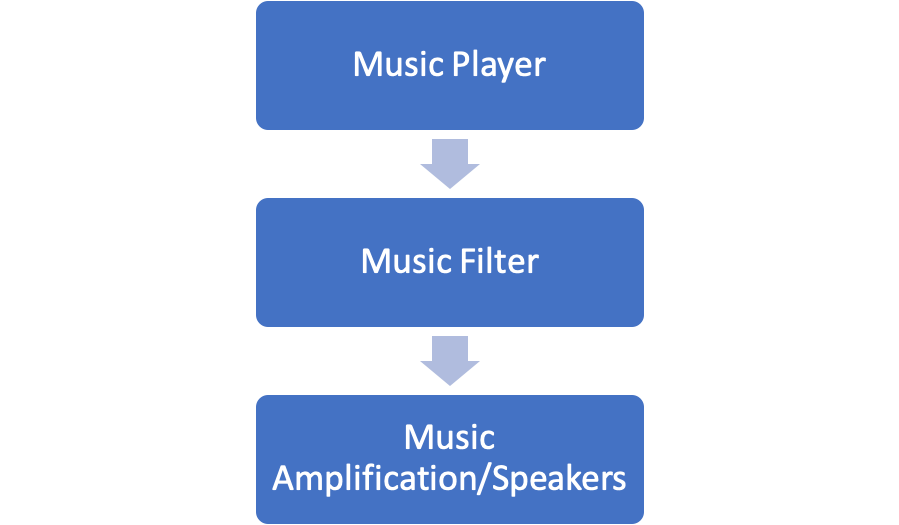
\includegraphics[width=0.60\textwidth]{images/layers}
 \caption{Architectural layer diagram of system}
\end{figure}

\subsection{Music Player Description}
The very first layer is responsible for producing the music. A website, seen and interacting with the raspberry pi, will play the music. Then, the music will be output through the raspberry pi's audio jack to the next layer. 

\subsection{Music Filter Description}
The second layer is where all the filtering happens. The music will first pass through a pre-amplifier which will amplify the signal to be heard through the speakers. Then the music will be separated by the different frequency ranges and sent to the next layer. 

\subsection{Audio Amplification/Speakers Description}
The last layer adjusts the intensity of the music to the users liking. Once the intensity is adjusted, the music will pass through the shakers on the different areas on the vest. 
